\subsection{Planeación}
En esta etapa, se estableció el propósito general de la investigación y se definieron las metas, así como las preguntas de investigación, métricas, criterios de clasificación, criterios de inclusión/exclusión y criterios de calidad de los estudios. Ver Figura~\ref{fig:etapa1}. \\

\begin{figure*}[tbp]
    \centering
    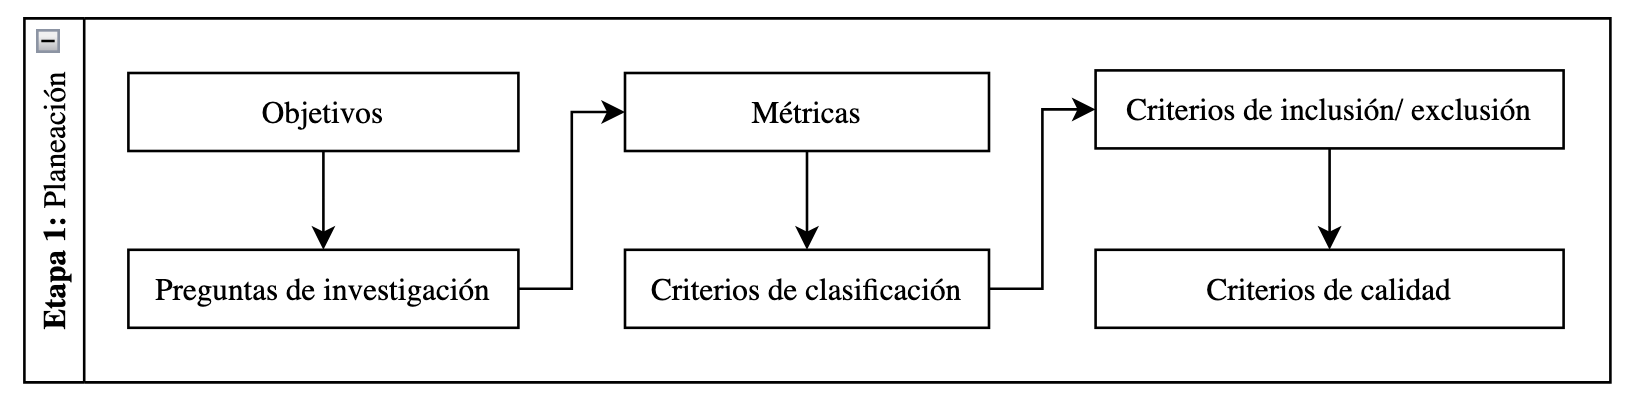
\includegraphics[width=0.8\textwidth]{resources/images/planeacion/etapa1.png}
    \caption{Composición de la etapa de planeación}\label{fig:etapa1}
\end{figure*}

\subsubsection{Objetivos}
\mbox{}\\
Teniendo en cuenta los aspectos descritos en la sección de motivación, se definieron 2 metas generales para la revisión sistemática de la literatura que se presentan en el cuadro~\ref{tab:metas}.

\begin{table}[htbp]
    \centering
    \begin{tabular}{>{\centering\arraybackslash}m{1cm} >{\arraybackslash}m{7cm}}
        \hline
        \textbf{Goal} & \textbf{Description} \\
        \hline
        M1 & Identificar trabajos relacionados con VBC en proyectos de docencia, investigación y extensión. \\
        \\
        M2 & Clasificar trabajos relacionados con VBC en los dominios de desarrollo de software, pensamiento computacional, computación paralela, análisis de datos, inteligencia artificial, redes computacionales, infraestructura de TI, HPC, entre otros. \\
        
        \hline
    \end{tabular}
    \caption{Metas del estudio}\label{tab:metas}
\end{table}





\subsubsection{Pregunta de investigación}
\mbox{}

\begin{table}[tbp]
    \scriptsize % reduce tamaño del texto
    \centering
    \renewcommand{\arraystretch}{1.3}
    \begin{tabularx}{\columnwidth}{>{\centering\arraybackslash}m{0.18\columnwidth} >{\RaggedRight\arraybackslash}X}
        \hline
        \textbf{Aspecto} & \textbf{Descripción} \\
        \hline
        Población & Trabajos relacionados con la VBC aplicadas en diversos dominios de TI con un énfasis en la educación, investigación y extensión. \\
        Intervención & Identificación y clasificación de los trabajos en VBC en los dominios de TI establecidos. \\
        Comparación & 
        1. Se comparan los proyectos que han hecho uso de la VBC para determinar cuáles han tenido mayor tasa de éxito expresado por los autores en cada dominio de TI. \newline
        2. Se analiza el impacto de la VBC en proyectos de docencia, investigación y extensión en comparación con otras soluciones tecnológicas. \\
        Salida & Estructura de clasificación de los trabajos relacionados con las VBC en cada dominio de TI que han impactado en proyectos de docencia, investigación y extensión. \\
        Contexto & Docencia, investigación y extensión con apropiación de los dominios de TI en forma de VBC. \\
        \hline
    \end{tabularx}
    \caption{Aspectos del modelo PICOC}\label{tab:PICOC}
\end{table}

\begin{table*}[!t]
\centering

\renewcommand{\arraystretch}{1.4}
\begin{tabularx}{\textwidth}{>{\centering\arraybackslash}m{0.05\textwidth} >{\centering\arraybackslash}m{0.05\textwidth} >{\RaggedRight\arraybackslash}X >{\RaggedRight\arraybackslash}X}
\toprule
\textbf{Meta} & \textbf{Pregunta} & \textbf{Descripción} & \textbf{Motivación} \\
\midrule
G1 & Q1 & ¿Cuáles son los trabajos relacionados con tecnologías de virtualización basadas en contenedores (VBC) que podrían impactar positivamente proyectos de docencia, investigación y extensión? & La transversalidad que ofrece la VBC, gracias a su reproducibilidad de entornos, permite estimular diferentes aristas de la sociedad. Su naturaleza facilita el transporte de soluciones de TI entre diferentes entornos, generando que una innovación en cualquier dominio social impacte directamente en otro. \\
\midrule
G2 & Q2 & ¿Cuáles son los principales trabajos relacionados con las tecnologías de virtualización basadas en contenedores (VBC) que podrían contribuir en los diversos dominios de TI, entre los que pueden ser desarrollo de software, pensamiento computacional, computación paralela, análisis de datos, inteligencia artificial, redes computacionales, infraestructura de TI, HPC, entre otros? & Se busca proporcionar una base sólida para investigadores, docentes y profesionales interesados en comprender el estado del arte actual en relación con las VBC, además del alcance y las aplicaciones de estos trabajos sin necesidad de un análisis profundo. \\
\bottomrule
\end{tabularx}
\caption{Preguntas de investigación y su motivación}
\label{tab:preguntas}
\end{table*}

Este modelo permite establecer los aspectos de ``Población'', ``Intervención'', ``Comparación'', ``Salida'' y ``Contexto'' que sirven para situar el trabajo a realizar. Ver cuadro~\ref{tab:PICOC}. \\
\\
Teniendo en cuenta el modelo PICOC, se definieron las preguntas de investigación. Ver cuadro~\ref{tab:preguntas}.\\

\subsubsection{Métricas}
\mbox{}\\

\begin{table}[htbp]
\centering
\renewcommand{\arraystretch}{1.3}
\begin{tabularx}{\columnwidth}{>{\centering\arraybackslash}m{0.15\textwidth} >{\RaggedRight\arraybackslash}X}
\toprule
\textbf{Métrica} & \textbf{Descripción} \\
\midrule
M1 & Cantidad de trabajos identificados en cada dominio de TI. \\
M2 & Cantidad de trabajos que están incluidos en educación. \\
M3 & Cantidad de trabajos que están incluidos en investigación. \\
M4 & Cantidad de trabajos que están incluidos en extensión. \\
\bottomrule
\end{tabularx}
\caption{Métricas definidas para el análisis}
\label{tab:metricas}
\end{table}

Se definieron las métricas del estudio usando un enfoque cuantitativo de acuerdo con la estructura de clasificación. Los detalles de las métricas se presentan en el cuadro~\ref{tab:metricas}.
Los criterios determinados limitaron la validez de los documentos a tres años, buscando la actualidad en el estudio. Además, el tipo se limitó a estudios primarios, buscando un rigor mayor en la revisión por pares.\\

\subsubsection{Tópicos de investigación}
\mbox{}\\
Las preguntas de investigación y el modelo PICOC sirven como línea base para definir los tópicos de investigación que se consideran relevantes para el estudio. Estos tópicos son: \textit{Container-based virtualization}, \textit{Education}, \textit{Research}, \textit{Industry}. 
La definición de los tópicos de investigación se realizó teniendo en cuenta los dominios de TI que se consideraron relevantes para el estudio.\\

\subsubsection{Criterios de inclusión y exclusión}
\mbox{}\\
\begin{table*}[!t]
\centering
\renewcommand{\arraystretch}{1.4}
\begin{tabularx}{\textwidth}{>{\centering\arraybackslash}m{0.15\textwidth} >{\RaggedRight\arraybackslash}X >{\RaggedRight\arraybackslash}X}
\toprule
\textbf{Categoría} & \textbf{Inclusión} & \textbf{Exclusión} \\
\midrule
Campos & Abstract & -- \\
\midrule
Tipo de publicación & Journal articles and conference proceedings & Thesis and book chapters \\
\midrule
Área/Disciplina & Management, Computer Science, Information Technology and Management, Engineering & Areas not related to virtualization, Computer Science, and Information Technology and Management \\
\midrule
Período & Between 2022 to 2024 & Less than 2022 \\
\midrule
Idioma & English & -- \\
\bottomrule
\end{tabularx}
\caption{Criterios de inclusión y exclusión}\label{tab:criterios}
\end{table*}

Los criterios de inclusión y exclusión se definieron para garantizar que los estudios seleccionados sean relevantes para las preguntas de investigación y los objetivos del estudio. Los criterios se presentan en el cuadro~\ref{tab:criterios}.
Se definió un período de 3 años en busca de la actualidad de los estudios. Además, se limitó los estudios a artículos de revistas buscando un mayor rigor en la revisión por pares. Los estudios deben estar escritos en inglés y en las áreas de \textit{Computer Science} y \textit{Management}, \textit{Information Technology and Management}, \textit{Engineering} en busca de la calidad de los estudios. Finalmente, se excluyeron los estudios que no están relacionados con la VBC, que no son revisados por pares o que no están disponibles en línea.\\

\subsubsection{Criterios de calidad}
\mbox{}\\
Para finalizar la etapa de planeación, se definieron tres criterios de calidad. \\

El primer criterio de calidad es una adaptación del CVI (Content Value Index)~\cite{almanasreh2019evaluation} y~\cite{yaghmaei2003content}.
En este caso, los artículos se evaluaron para determinar si cumplen con los criterios de inclusión y exclusión definidos y si son relevantes para las preguntas de investigación. Se usó una escala cuantitativa de 0 a 5, donde 0 indica una baja relación con las metas del SMS y 5 indica una alta relación.
Ver formula~\ref{eq:cvi}. En esta formula, K es el número impar de evaluadores y f(n) es la frecuencia de respuestas para cada valor de la escala.\\

\begin{equation}
\label{eq:cvi}
CVI = \frac{\sum_{n=1}^{k} f(n)}{k}
\end{equation}

El segundo criterio de calidad es el número de citas de cada estudio de acuerdo con la fecha de publicación (A), el cual se denomina SCI (Scientific Citation Index). Ver formula~\ref{eq:sci}. En esta formula, C es el número de citas entre 2022 y 2024 y A es el tiempo de publicación del estudio. Así, un artículo publicado en 2024 con las misma cantidad de citas que un artículo publicado en 2022 tendrá un SCI más alto.\\

\begin{equation}
\label{eq:sci}
SCI = \frac{C}{A}
\end{equation}

El tercer criterio de calidad corresponde a la relación de los estudios con las preguntas de investigación. Este criterio se denomina IRRQ (Indice de relación con las preguntas de investigación). Ver formula~\ref{eq:irrq}. 

\begin{equation}
\label{eq:irrq}
IRRQ = \frac{N}{2}
\end{equation}

N corresponde al número de preguntas de investigación que el estudio responde. Este valor se divide en 2 porque es el número de preguntas de investigación definidas en la etapa de planeación. \\